\definecolor{c82b366}{RGB}{130,179,102}
\definecolor{cd5e8d4}{RGB}{213,232,212}
\definecolor{c666666}{RGB}{102,102,102}
\definecolor{whitesmoke}{RGB}{245,245,245}
\definecolor{c333333}{RGB}{51,51,51}
\definecolor{c6c8ebf}{RGB}{108,142,191}
\definecolor{cdae8fc}{RGB}{218,232,252}


\def \globalscale {0.900000}
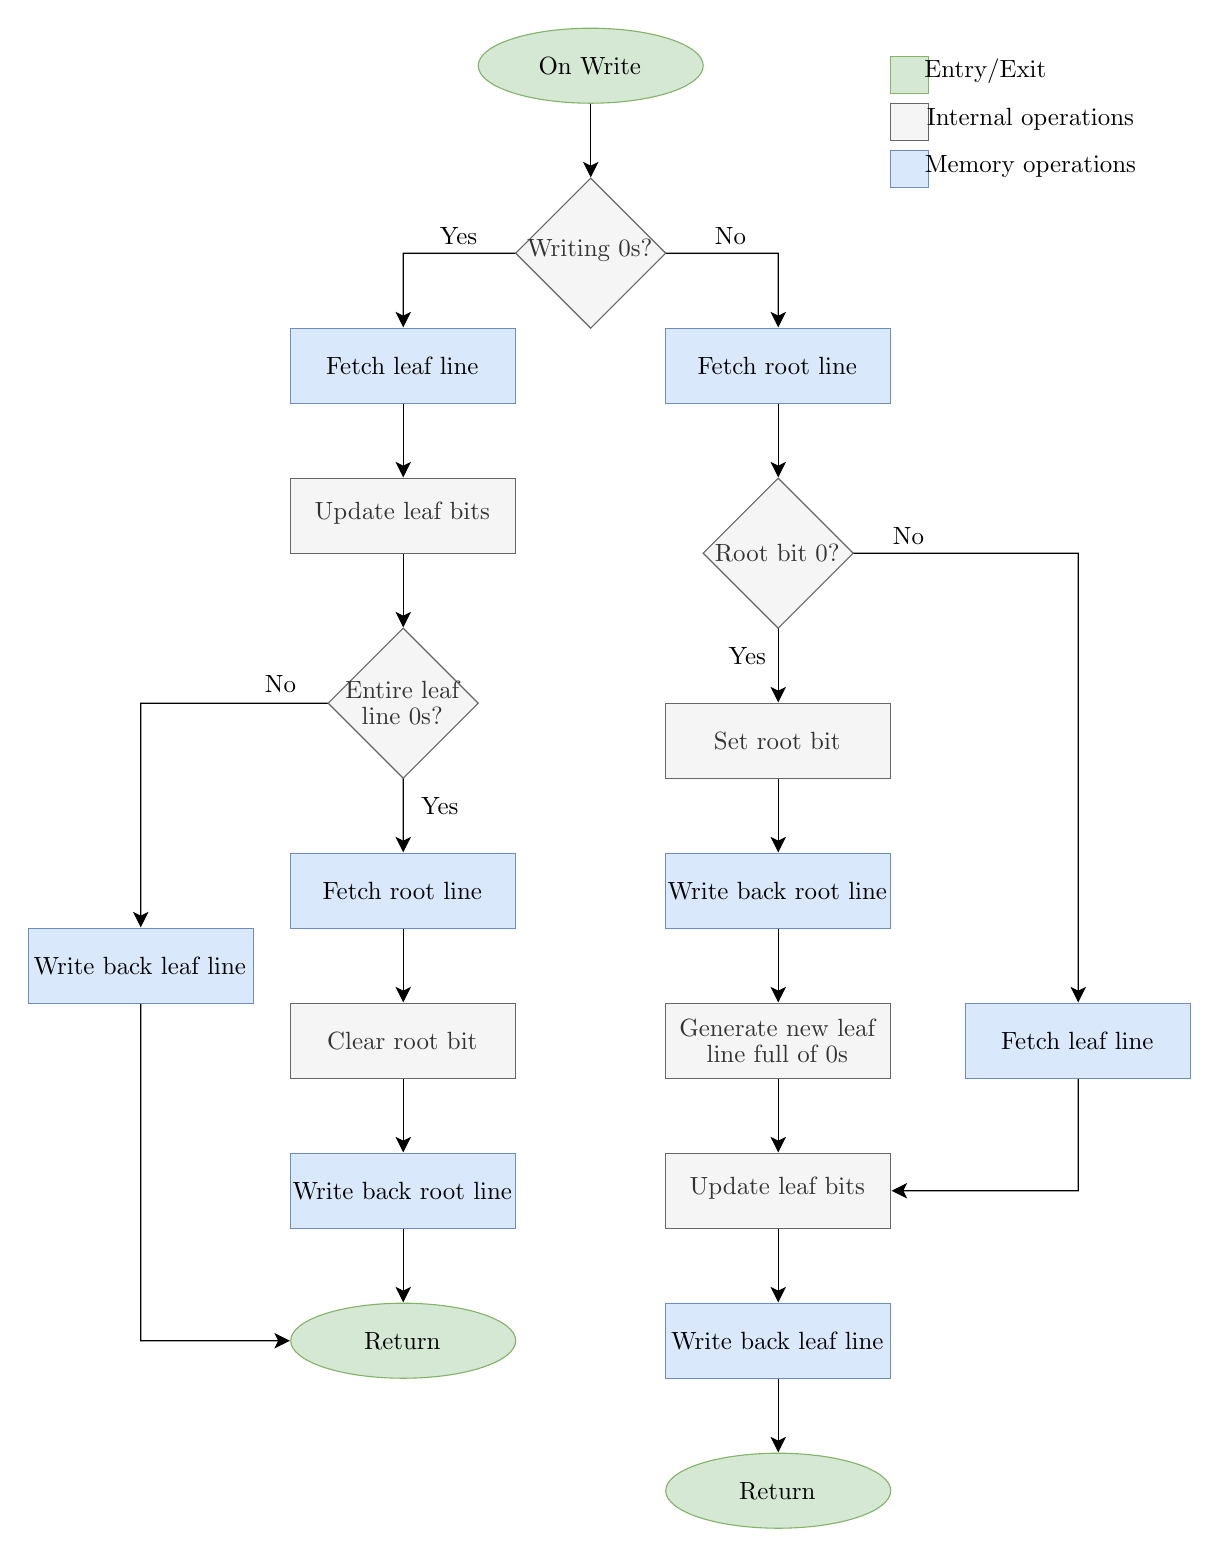
\begin{tikzpicture}[y=1cm, x=1cm, yscale=\globalscale,xscale=\globalscale, every node/.append style={scale=\globalscale}, inner sep=0pt, outer sep=0pt]
  \path[draw=black,miter limit=10.0] (7.9375, 20.1348) -- (7.9375, 19.245);



  \path[draw=black,fill=black,miter limit=10.0] (7.9375, 19.1061) -- (7.8449, 19.2913) -- (7.9375, 19.245) -- (8.0301, 19.2913) -- cycle;



  \path[draw=c82b366,fill=cd5e8d4] (7.9375, 20.664) ellipse (1.5875cm and 0.5292cm);



  \begin{scope}[fill=black,anchor=south]
    \node[text=black,anchor=south] (text6531) at (7.9243, 20.5449){On Write};



  \end{scope}
  \path[draw=black,miter limit=10.0] (6.88, 18.0173) -- (5.2925, 18.0173) -- (5.2917, 17.1283);



  \path[draw=black,fill=black,miter limit=10.0] (5.2917, 16.9894) -- (5.1993, 17.1746) -- (5.2917, 17.1283) -- (5.3845, 17.1746) -- cycle;



  \path[draw=black,miter limit=10.0] (8.995, 18.0173) -- (10.5841, 18.0173) -- (10.5833, 17.1283);



  \path[draw=black,fill=black,miter limit=10.0] (10.5833, 16.9894) -- (10.491, 17.1746) -- (10.5833, 17.1283) -- (10.6762, 17.1746) -- cycle;



  \path[draw=c666666,fill=whitesmoke,miter limit=10.0] (7.9375, 19.0765) -- (8.9958, 18.0181) -- (7.9375, 16.9598) -- (6.8792, 18.0181) -- cycle;



  \begin{scope}[fill=c333333,anchor=south]
    \node[text=c333333,anchor=south] (text4698) at (7.9243, 17.8991){Writing 0s?};



  \end{scope}
  \path[draw=black,miter limit=10.0] (5.2917, 15.9015) -- (5.2917, 15.0117);



  \path[draw=black,fill=black,miter limit=10.0] (5.2917, 14.8728) -- (5.1991, 15.058) -- (5.2917, 15.0117) -- (5.3843, 15.058) -- cycle;



  \path[draw=c6c8ebf,fill=cdae8fc] (3.7042, 16.9598) rectangle (6.8792, 15.9015);



  \begin{scope}[fill=black,anchor=south]
    \node[text=black,anchor=south] (text9934) at (5.2784, 16.3116){Fetch leaf line};



  \end{scope}
  \path (5.2917, 18.6531) rectangle (6.8792, 17.8594);



  \begin{scope}[fill=black,anchor=south]
    \node[text=black,anchor=south] (text3774) at (6.0722, 18.1372){Yes};



  \end{scope}
  \path[draw=black,miter limit=10.0] (5.2917, 13.7848) -- (5.2917, 12.895);



  \path[draw=black,fill=black,miter limit=10.0] (5.2917, 12.7561) -- (5.1991, 12.9413) -- (5.2917, 12.895) -- (5.3843, 12.9413) -- cycle;



  \path[draw=c666666,fill=whitesmoke] (3.7042, 14.8431) rectangle (6.8792, 13.7848);



  \begin{scope}[fill=c333333,anchor=south]
    \node[text=c333333,anchor=south] (text3459) at (5.2784, 14.1949){Update leaf bits};



  \end{scope}
  \path[draw=black,miter limit=10.0] (1.5883, 7.4348) -- (1.5883, 2.6715) -- (3.5356, 2.6723);



  \path[draw=black,fill=black,miter limit=10.0] (3.6745, 2.6723) -- (3.4893, 2.5797) -- (3.5356, 2.6723) -- (3.4893, 2.7649) -- cycle;



  \path[draw=c6c8ebf,fill=cdae8fc] (0.0, 8.4931) rectangle (3.175, 7.4348);



  \begin{scope}[fill=black,anchor=south]
    \node[text=black,anchor=south] (text7725) at (1.5743, 7.8449){Write back leaf line};



  \end{scope}
  \path[draw=black,miter limit=10.0] (5.2925, 10.6106) -- (5.2925, 10.0798) -- (5.2919, 9.72);



  \path[draw=black,fill=black,miter limit=10.0] (5.2917, 9.5811) -- (5.1993, 9.7663) -- (5.2919, 9.72) -- (5.3845, 9.766) -- cycle;



  \path[draw=black,miter limit=10.0] (4.2341, 11.6673) -- (1.5883, 11.6673) -- (1.5875, 8.6617);



  \path[draw=black,fill=black,miter limit=10.0] (1.5875, 8.5228) -- (1.4949, 8.708) -- (1.5875, 8.6617) -- (1.6801, 8.708) -- cycle;



  \path[draw=c666666,fill=whitesmoke,miter limit=10.0] (5.2917, 12.7265) -- (6.35, 11.6681) -- (5.2917, 10.6098) -- (4.2333, 11.6681) -- cycle;



  \begin{scope}[fill=c333333,anchor=south]
    \node[text=c333333,anchor=south] (text1713) at (5.2784, 11.7343){Entire leaf};



    \node[text=c333333,anchor=south] (text2787) at (5.2784, 11.3639){line 0s?};



  \end{scope}
  \path[draw=black,miter limit=10.0] (5.2917, 8.4931) -- (5.2917, 7.6033);



  \path[draw=black,fill=black,miter limit=10.0] (5.2917, 7.4644) -- (5.1991, 7.6496) -- (5.2917, 7.6033) -- (5.3843, 7.6496) -- cycle;



  \path[draw=c6c8ebf,fill=cdae8fc] (3.7042, 9.5515) rectangle (6.8792, 8.4931);



  \begin{scope}[fill=black,anchor=south]
    \node[text=black,anchor=south] (text2040) at (5.2784, 8.9032){Fetch root line};



  \end{scope}
  \path[draw=black,miter limit=10.0] (5.2917, 6.3765) -- (5.2917, 5.4867);



  \path[draw=black,fill=black,miter limit=10.0] (5.2917, 5.3478) -- (5.1991, 5.533) -- (5.2917, 5.4867) -- (5.3843, 5.533) -- cycle;



  \path[draw=c666666,fill=whitesmoke] (3.7042, 7.4348) rectangle (6.8792, 6.3765);



  \begin{scope}[fill=c333333,anchor=south]
    \node[text=c333333,anchor=south] (text4453) at (5.2784, 6.7866){Clear root bit};



  \end{scope}
  \path[draw=black,miter limit=10.0] (5.2917, 4.2598) -- (5.2917, 3.37);



  \path[draw=black,fill=black,miter limit=10.0] (5.2917, 3.2311) -- (5.1991, 3.4163) -- (5.2917, 3.37) -- (5.3843, 3.4163) -- cycle;



  \path[draw=c6c8ebf,fill=cdae8fc] (3.7042, 5.3181) rectangle (6.8792, 4.2598);



  \begin{scope}[fill=black,anchor=south]
    \node[text=black,anchor=south] (text7428) at (5.2784, 4.6699){Write back root line};



  \end{scope}
  \path[draw=c82b366,fill=cd5e8d4] (5.2917, 2.6723) ellipse (1.5875cm and 0.5292cm);



  \begin{scope}[fill=black,anchor=south]
    \node[text=black,anchor=south] (text7087) at (5.2784, 2.5532){Return};



  \end{scope}
  \path (5.2917, 10.4775) rectangle (6.35, 9.9483);



  \begin{scope}[fill=black,anchor=south]
    \node[text=black,anchor=south] (text6202) at (5.8076, 10.0939){Yes};



  \end{scope}
  \path (3.175, 12.1973) rectangle (3.9688, 11.6681);



  \begin{scope}[fill=black,anchor=south]
    \node[text=black,anchor=south] (text4707) at (3.5586, 11.8136){No};



  \end{scope}
  \path[draw=black,miter limit=10.0] (10.5833, 15.9015) -- (10.5833, 15.0117);



  \path[draw=black,fill=black,miter limit=10.0] (10.5833, 14.8728) -- (10.4907, 15.058) -- (10.5833, 15.0117) -- (10.6759, 15.058) -- cycle;



  \path[draw=c6c8ebf,fill=cdae8fc] (8.9958, 16.9598) rectangle (12.1708, 15.9015);



  \begin{scope}[fill=black,anchor=south]
    \node[text=black,anchor=south] (text1959) at (10.5701, 16.3116){Fetch root line};



  \end{scope}
  \path (9.525, 18.5208) rectangle (10.3188, 17.9917);



  \begin{scope}[fill=black,anchor=south]
    \node[text=black,anchor=south] (text4503) at (9.9086, 18.1372){No};



  \end{scope}
  \path[draw=black,miter limit=10.0] (10.5833, 12.7265) -- (10.5833, 11.8367);



  \path[draw=black,fill=black,miter limit=10.0] (10.5833, 11.6978) -- (10.4907, 11.883) -- (10.5833, 11.8367) -- (10.6759, 11.883) -- cycle;



  \path[draw=black,miter limit=10.0] (11.6409, 13.784) -- (14.8175, 13.784) -- (14.8167, 7.6033);



  \path[draw=black,fill=black,miter limit=10.0] (14.8167, 7.4644) -- (14.7241, 7.6496) -- (14.8167, 7.6033) -- (14.9093, 7.6496) -- cycle;



  \path[draw=c666666,fill=whitesmoke,miter limit=10.0] (10.5833, 14.8431) -- (11.6417, 13.7848) -- (10.5833, 12.7265) -- (9.525, 13.7848) -- cycle;



  \begin{scope}[fill=c333333,anchor=south]
    \node[text=c333333,anchor=south] (text7143) at (10.5701, 13.6657){Root bit 0?};



  \end{scope}
  \path[draw=black,miter limit=10.0] (10.5833, 10.6098) -- (10.5833, 9.72);



  \path[draw=black,fill=black,miter limit=10.0] (10.5833, 9.5811) -- (10.4907, 9.7663) -- (10.5833, 9.72) -- (10.6759, 9.7663) -- cycle;



  \path[draw=c666666,fill=whitesmoke] (8.9958, 11.6681) rectangle (12.1708, 10.6098);



  \begin{scope}[fill=c333333,anchor=south]
    \node[text=c333333,anchor=south] (text556) at (10.5701, 11.0199){Set root bit};



  \end{scope}
  \path[draw=black,miter limit=10.0] (10.5833, 8.4931) -- (10.5833, 7.6033);



  \path[draw=black,fill=black,miter limit=10.0] (10.5833, 7.4644) -- (10.4907, 7.6496) -- (10.5833, 7.6033) -- (10.6759, 7.6496) -- cycle;



  \path[draw=c6c8ebf,fill=cdae8fc] (8.9958, 9.5515) rectangle (12.1708, 8.4931);



  \begin{scope}[fill=black,anchor=south]
    \node[text=black,anchor=south] (text3310) at (10.5701, 8.9032){Write back root line};



  \end{scope}
  \path[draw=black,miter limit=10.0] (10.5833, 6.3765) -- (10.5833, 5.4867);



  \path[draw=black,fill=black,miter limit=10.0] (10.5833, 5.3478) -- (10.4907, 5.533) -- (10.5833, 5.4867) -- (10.6759, 5.533) -- cycle;



  \path[draw=c666666,fill=whitesmoke] (8.9958, 7.4348) rectangle (12.1708, 6.3765);



  \begin{scope}[fill=c333333,anchor=south]
    \node[text=c333333,anchor=south] (text449) at (10.5701, 6.9718){Generate new leaf};



    \node[text=c333333,anchor=south] (text5075) at (10.5701, 6.6014){line full of 0s};



  \end{scope}
  \path[draw=black,miter limit=10.0] (10.5833, 4.2598) -- (10.5833, 3.37);



  \path[draw=black,fill=black,miter limit=10.0] (10.5833, 3.2311) -- (10.4907, 3.4163) -- (10.5833, 3.37) -- (10.6759, 3.4163) -- cycle;



  \path[draw=c666666,fill=whitesmoke] (8.9958, 5.3181) rectangle (12.1708, 4.2598);



  \begin{scope}[fill=c333333,anchor=south]
    \node[text=c333333,anchor=south] (text9030) at (10.5701, 4.6699){Update leaf bits};



  \end{scope}
  \path[draw=black,miter limit=10.0] (10.5833, 2.1431) -- (10.5833, 1.2533);



  \path[draw=black,fill=black,miter limit=10.0] (10.5833, 1.1144) -- (10.4907, 1.2996) -- (10.5833, 1.2533) -- (10.6759, 1.2996) -- cycle;



  \path[draw=c6c8ebf,fill=cdae8fc] (8.9958, 3.2015) rectangle (12.1708, 2.1431);



  \begin{scope}[fill=black,anchor=south]
    \node[text=black,anchor=south] (text7966) at (10.5701, 2.5532){Write back leaf line};



  \end{scope}
  \path[draw=c82b366,fill=cd5e8d4] (10.5833, 0.5556) ellipse (1.5875cm and 0.5292cm);



  \begin{scope}[fill=black,anchor=south]
    \node[text=black,anchor=south] (text2631) at (10.5701, 0.4366){Return};



  \end{scope}
  \path (9.3663, 12.7265) rectangle (10.9538, 11.9327);



  \begin{scope}[fill=black,anchor=south]
    \node[text=black,anchor=south] (text5207) at (10.1468, 12.2105){Yes};



  \end{scope}
  \path[draw=black,miter limit=10.0] (14.8175, 6.3765) -- (14.8175, 4.7882) -- (12.3394, 4.789);



  \path[draw=black,fill=black,miter limit=10.0] (12.2005, 4.789) -- (12.3857, 4.8816) -- (12.3394, 4.789) -- (12.3857, 4.6964) -- cycle;



  \path[draw=c6c8ebf,fill=cdae8fc] (13.2292, 7.4348) rectangle (16.4042, 6.3765);



  \begin{scope}[fill=black,anchor=south]
    \node[text=black,anchor=south] (text9530) at (14.8034, 6.7866){Fetch leaf line};



  \end{scope}
  \path (11.6417, 14.4198) rectangle (13.2292, 13.626);



  \begin{scope}[fill=black,anchor=south]
    \node[text=black,anchor=south] (text6839) at (12.4222, 13.9039){No};



  \end{scope}
  \path[draw=c82b366,fill=cd5e8d4] (12.1708, 20.7963) rectangle (12.7, 20.2671);



  \path (12.5942, 20.9285) rectangle (14.4463, 20.1348);



  \begin{scope}[fill=black,anchor=south]
    \node[text=black,anchor=south] (text1427) at (13.507, 20.4126){Entry/Exit};



  \end{scope}
  \path[draw=c666666,fill=whitesmoke] (12.1708, 20.1348) rectangle (12.7, 19.6056);



  \path (12.5677, 20.2671) rectangle (15.7427, 19.4733);



  \begin{scope}[fill=black,anchor=south]
    \node[text=black,anchor=south] (text7392) at (14.142, 19.7511){Internal operations};



  \end{scope}
  \path[draw=c6c8ebf,fill=cdae8fc] (12.1708, 19.4733) rectangle (12.7, 18.9442);



  \path (12.4354, 19.6056) rectangle (15.875, 18.8119);



  \begin{scope}[fill=black,anchor=south]
    \node[text=black,anchor=south] (text9036) at (14.142, 19.0897){Memory operations};



  \end{scope}

\end{tikzpicture}
